\capitulo{5}{Aspectos relevantes del desarrollo del proyecto}

En este apartado se va a comentar, a manera de resumen temporal, el desarrollo del proyecto. Es en este apartado donde se comentarán las opciones y decisiones tomadas, los problemas surgidos y todos los aspectos importantes. Se ha considerado que la mejor forma de organizar este apartado es en seccionaes donde se comenta cada apartado del desarrollo.

\section{Desarrollo FIS-HUBU}\label{desarrolloFH}
FIS-HUBU es una aplicación web que permite realizar vídeo llamadas entre responsables y pacientes con Parkinson para realizar rehabilitaciones de manera \textit{online}, es decir, sin la necesidad de desplazarse hasta la consulta o el hospital. Esta aplicación, que ha sido desarrollada junto con mi compañero José Luis Garrido Labrador, permite por parte del responsable observar y evaluar la evolución del estado de un paciente, esta evolución también es visible para el paciente que puede ver su propio progreso.

La aplicación puede dividirse en distintas partes que serán comentadas a continuación.
\subsection{Vídeo llamadas}
El punto principal de la aplicación, y por ende su principal uso, son las vídeo llamadas entre pacientes y responsables o terapeutas que permitan sustituir la rehabilitaciones presenciales en consulta por rehabilitaciones \textit{online}, permitiendo así que estás se puedan dar más a menudo y puedan ser accesibles para un mayor número de personas, sobre todo para aquellos pacientes que no se pueden desplazar.

Primero se realizó una investigación sobre las principales plataformas de vídeo llamadas. Lo que se estaba buscando de estas plataformas era:
\begin{itemize}
	\item Creación de llamadas de manera sencilla y automática. Si es posible a partir de url.
	\item Vídeo llamada estable sin necesidad de una gran conexión.
	\item Plataforma que permita grabar la cámara de los pacientes.
	\item Plataforma gratuita.
\end{itemize}

Dentro de las plataformas que se investigaron están las más conocidas aplicaciones de este tipo como puede ser \textit{Skype}, pero al final se decidió utilizar \textit{Jitsi} ya que proporciona todas las necesidades anteriormente comentadas, y además permite en un futuro poder crear un servidor propio donde poder modificar parámetros como la calidad de las llamadas.

\subsection{Responsable}
Parte de la aplicación donde los responsables pueden realizar las siguientes tareas:
\begin{itemize}
	\item Iniciar un vídeo llamada con un paciente.
	\item Evaluar la evolución de los pacientes.
	\item Modificar las evaluaciones de los pacientes.
	\item Comprobar la evolución de los pacientes.
\end{itemize}

La interfaz de la aplicación para tipo de usuario es sencilla y clara, como se puede ver en el menú principal, figura~\ref{fig:menuPaciente}, o en el menú de estadísticas, figuras~\ref{fig:menuest} y~\ref{fig:ejemploest}.

\begin{figure}[h]
	\centering
	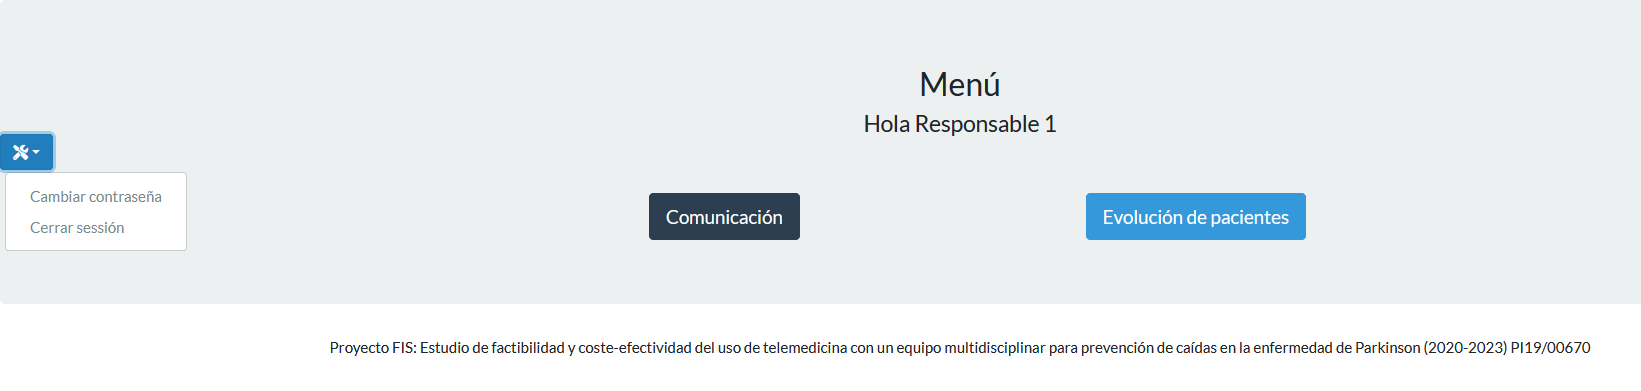
\includegraphics[width=1\textwidth]{menuResponsable}
	\caption{Menú principal de un responsable.}
	\label{fig:menuPaciente}
\end{figure}

\begin{figure}[h]
	\centering
	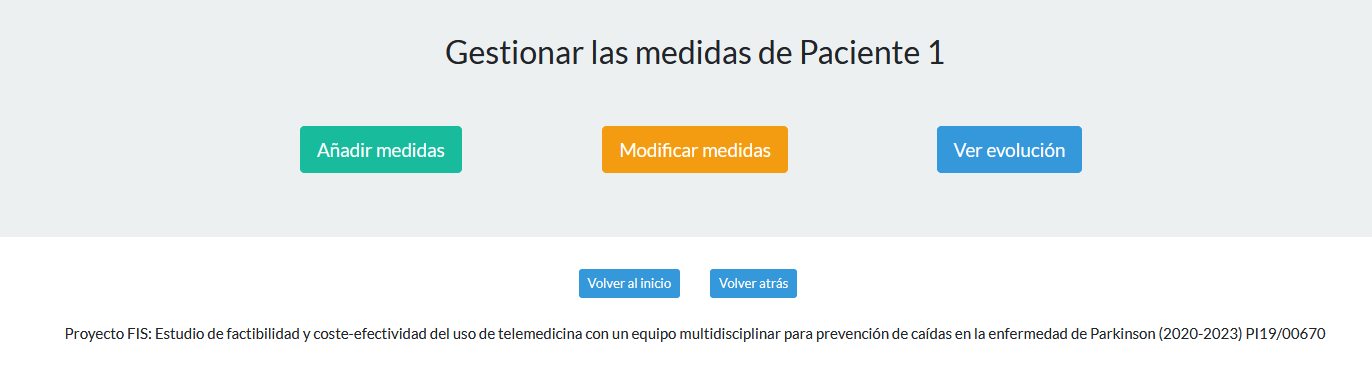
\includegraphics[width=1\textwidth]{menuestad}
	\caption{Menú de estadísticas.}
	\label{fig:menuest}
\end{figure}

\begin{figure}[h]
	\centering
	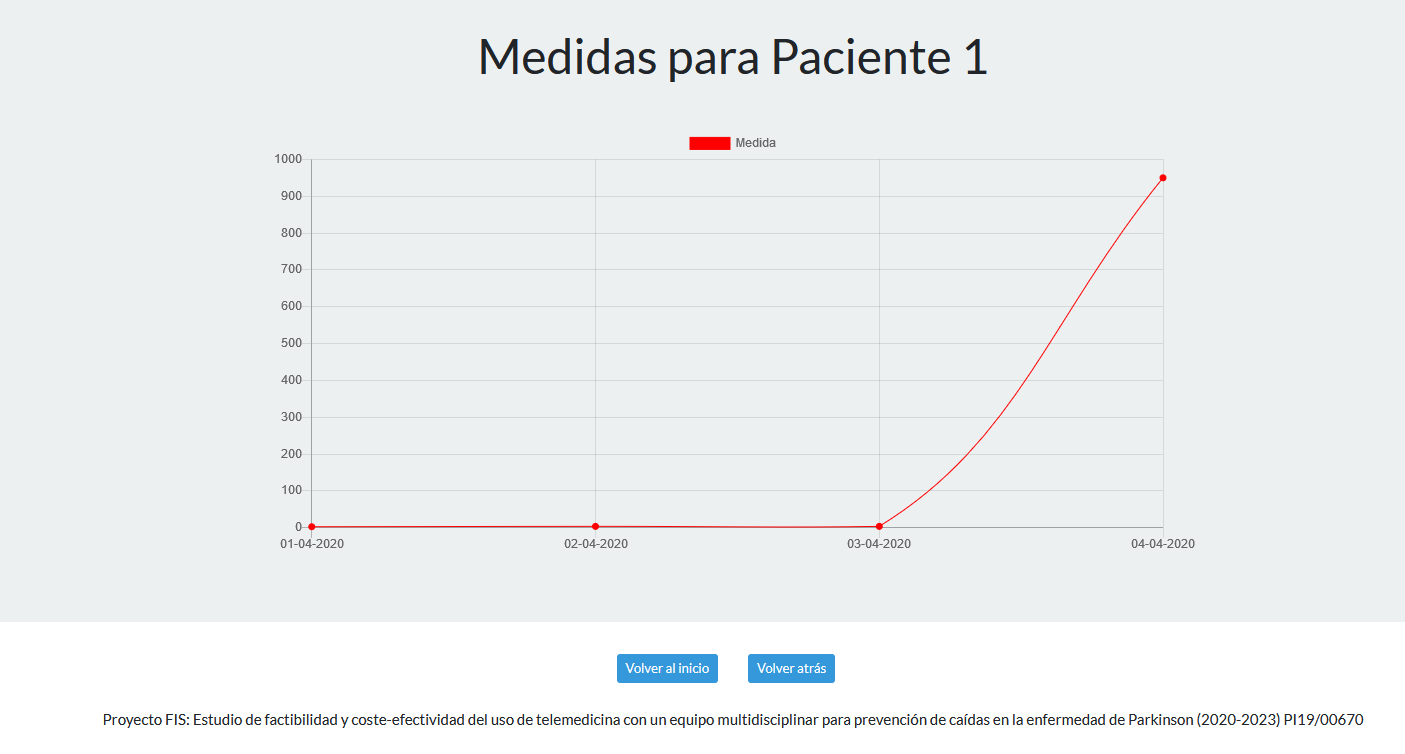
\includegraphics[width=1\textwidth]{ejemploest}
	\caption{Ejemplo de la evolución de un paciente vista por un responsable.}
	\label{fig:ejemploest}
\end{figure}

\subsection{Paciente}
Los pacientes que van a utilizar la aplicación, son pacientes mayores con Parkinson. Esto se ha tenido muy en cuenta tanto en el diseño como en la creación de la parte de la aplicación orientada en los pacientes, se ha intentado que esta parte sea lo más accesible posible, para que todos los pacientes puedan manejarse bien con la aplicación y así poder sacarle el mayor provecho.

Para poder realizar una aplicación lo más accesible posible primero se ha de saber la forma que van a tener los pacientes de interactuar con ésta. En este caso los pacientes van a utilizar un mando de SNES\footnote{SNES: \textit{Super Nintendo Entertainment System}} con botones de colores, es por ello que se ha aprovechado estos colores para poder mostrar en la interfaz de la aplicación que botón han de pulsar para realizar que acción. Además, se ha creado un botón de ayuda que carga una página donde se puede ver la acción que realiza cada botón del mando. Un ejemplo de la interfaz de esta aplicación se puede ver en la figura~\ref{fig:menupaciente}.

\begin{figure}[h]
	\centering
	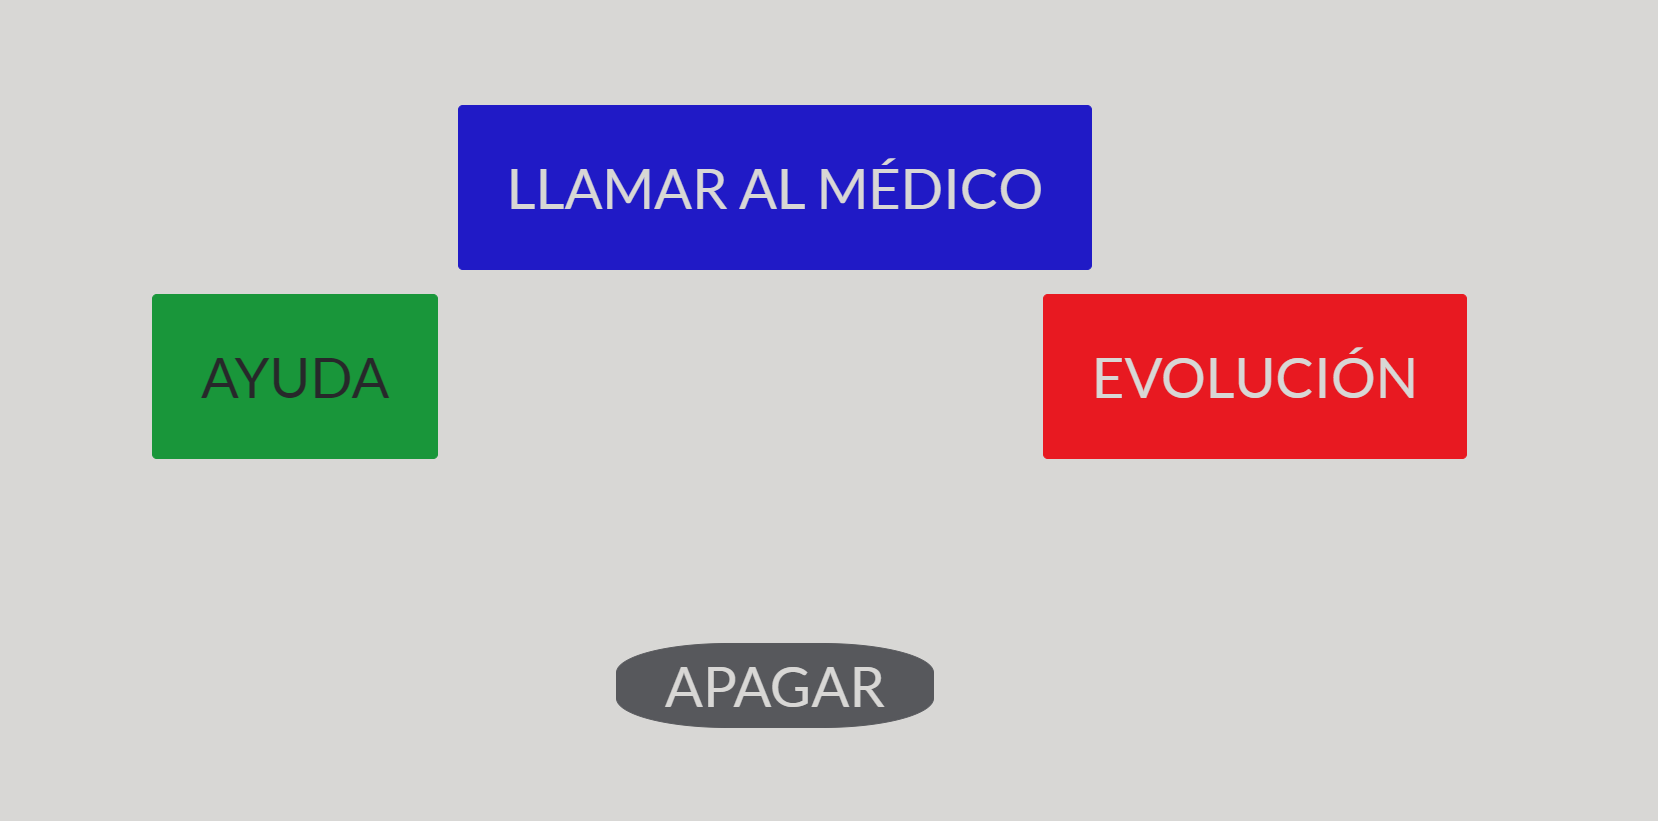
\includegraphics[width=1\textwidth]{menupac}
	\caption{Menú principal de los pacientes.}
	\label{fig:menupaciente}
\end{figure}

\subsection{Dispositivos necesarios}
Para poder utilizar la aplicación se necesitan distintos dispositivos, que dependiendo del tipo de usuario (responsable o paciente) son unos u otros.

Para los responsables lo único que se necesita es un ordenador con conexión a \textit{Internet} y una cámara conectada a éste.

Por otro lado, los pacientes se presupone que no disponen de ningún dispositivo capaz de cargar la aplicación, es por ello que a cada paciente se le proporciona:
\begin{itemize}
	\item MSI
	\item CAMARA
\end{itemize}

\subsection{Conexión}
Como ya se ha comentado, el principal uso de la aplicación es las rehabilitaciones \textit{online} para pacientes, mayoritariamente de tercera edad, que no se pueden desplazar a las consultas. Muchas de estas personas mayores viven en lugares donde no se tiene contratada ninguna línea de \textit{Internet}, es por ello que además del desarrollo de la aplicación se contrató una serie de \textit{routers} 4G para poder proporcionar conexión a los dispositivos necesarios. 

\section{Investigación algoritmos de visión por computador}
Tras haber desarrollado la versión inicial, donde en un futuro se quiere añadir lo resultados de este proyecto, se pasó a realizar la primera investigación sobre los distintos algoritmos de visión por computar capaces de detectar y seguir los movimientos de una persona. 

De estos algoritmos se necesita:
\begin{itemize}
	\item Posibilidad de cargar un modelo existente o crear un modelo capaz de detectar a la persona que sale en la imagen.
	\item Posibilidad de cargar un modelo existente o crear un modelo capaz de detectar la posición de la persona.
	\item Que el procesado de nuevos fotogramas para detectar a la persona y su posición se realicé en poco tiempo.
	\item Que la salida del procesado de los fotogramas pueda servir para una posterior comparación con el ejercicio base.
\end{itemize}

Teniendo todos estos factores en cuenta se estudió qué herramientas se pueden usar para esta fase del trabajo. Se buscó herramientas programadas en \textit{Python} para poder conectarse bien con el resto del proyecto y porque es uno de los lenguajes con los cuales se tiene más soltura, tanto por parte del alumno como por parte de los tutores para resolver dudas y ayudar en los problemas. Las herramientas encontradas fuera:
\begin{itemize}
	\item \textit{TF-Pose-Estimator}.
	\item \textit{PoseNet}.
	\item \textit{Detectron2}.
\end{itemize}

De cada una de estas herramientas se realizó una investigación y experimentación para probar si cumplían las necesidades requeridas. Al finalizar esta etapa, la única herramienta que permitía realizar todas las necesidades era \textit{Detectron2}. Además, permite con un modelo ya creado por los propios desarrolladores realizar las tareas de predicción de elementos y de la posición de la persona.

Cabe destacar uno de los grandes problemas que surgió en esta fase, y fue justamente con \textit{Detectron2}, la herramienta elegida. El problema era que las versiones de \textit{CUDA} y de \textit{PyTorch} no eran compatible. El problema se agrandó al estar trabajando en un \textit{workstation} de la universidad como es \textit{Gamma} que utilizan otros investigadores y también por la compleja estructura del propio computador. Tras hablar con el administrador de la computadora, que es uno de los tutores de este trabajo, el doctor Álvar Arnaiz Gonzalez, se pudo arreglar el problema actualizando la versión de los \textit{drivers} de \textit{CUDA}, y una vez actualizados descargando la versión compatible de \textit{PyTorch}. 
\section{Investigación de \textit{Detectron2}}
La fase de investigación de \textit{Detectron2} fue una de las más importantes, y por ende, más costosas en tiempo. Fue en esta fase donde se investigaron las distintas formas que tiene la herramienta para crear o importar modelos con los que poder trabajar. Una vez se seleccionó el modelo se realizó otro estudio para ver que configuración era la más correcta en el problema tratado.

Al ser una de las fases en las que más tiempo se ha dedicado, también es una de las fases donde surgieron más problemas tanto en la creación de los modelos, como en la visualización y el almacenamiento de los resultados obtenidos. Todos estos problemas serán comentados en este apartado.  
\subsection{Selección del modelo}
Tras haber elegido a \textit{Detrectron2} como herramienta de visión por computador para capturar detectar a los pacientes y obtener de estos sus posiciones, elegir qué modelo, dentro de las posibilidades de la herramienta, utilizar para realizar estás tareas.

\textit{Dectectron2} permite dos formas de obtener un modelo:
\begin{itemize}
	\item Crear un modelo propio a partir de una gran cantidad de datos.
	\item Importación de modelos ya entrenados.
\end{itemize}

Ante la falta de datos para la creación de un modelo que diese buenos resultados, y al comprobar en la fase anterior que con la importación de modelos existentes se podían obtener buenos resultados la investigación se centró en los modelos ya existentes realizados por los creados de la herramienta. Estos modelos de redes neuronales fueron entrenados en servidores \textit{Big Basin} de \textit{Facebook}, sucesores de los servidores \textit{Big Sur}, ambos orientados al uso de arquitecturas con varias GPUs potentes para el entrenamiento y uso de algoritmos de inteligencia artificial~\cite{bigbasin}. En concreto, estos modelos fueron entrenados con 8 Nvidia Tesla V100 con \textit{NVLink}, un tecnología que mejorar las interconexiones entre GPUs proporcionando mayor ancho de banda, haciendo el sistema más escalable~\cite{nvlink}. La mejora con otras generaciones de comunicación \textit{inter-GPU} se puede ver en la figura~\ref{fig:nvlink}.

\begin{figure}[h]
	\centering
	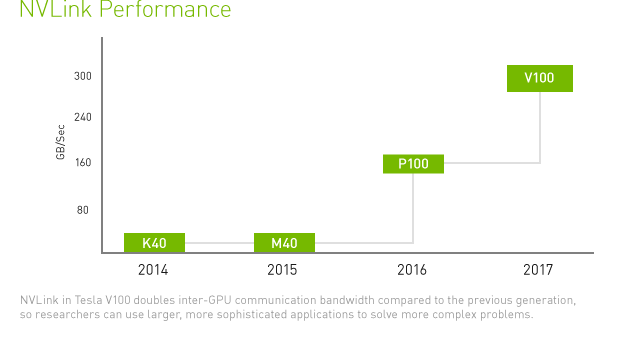
\includegraphics[width=1\textwidth]{nvlink}
	\caption{Mejora del rendimiento en GB/s con NVlink~\cite{nvlink}.}
	\label{fig:nvlink}
\end{figure}

Los modelos creados en \textit{Detectron2} se diferencian en los siguientes tipos:
\begin{itemize}
	\item COCO Detection with Faster R-CNN (Figura~\ref{fig:faster_rcnn_R_50_C4_1x}): modelos que predice los objetos y personas de la imagen.
	\begin{figure}[h]
		\centering
		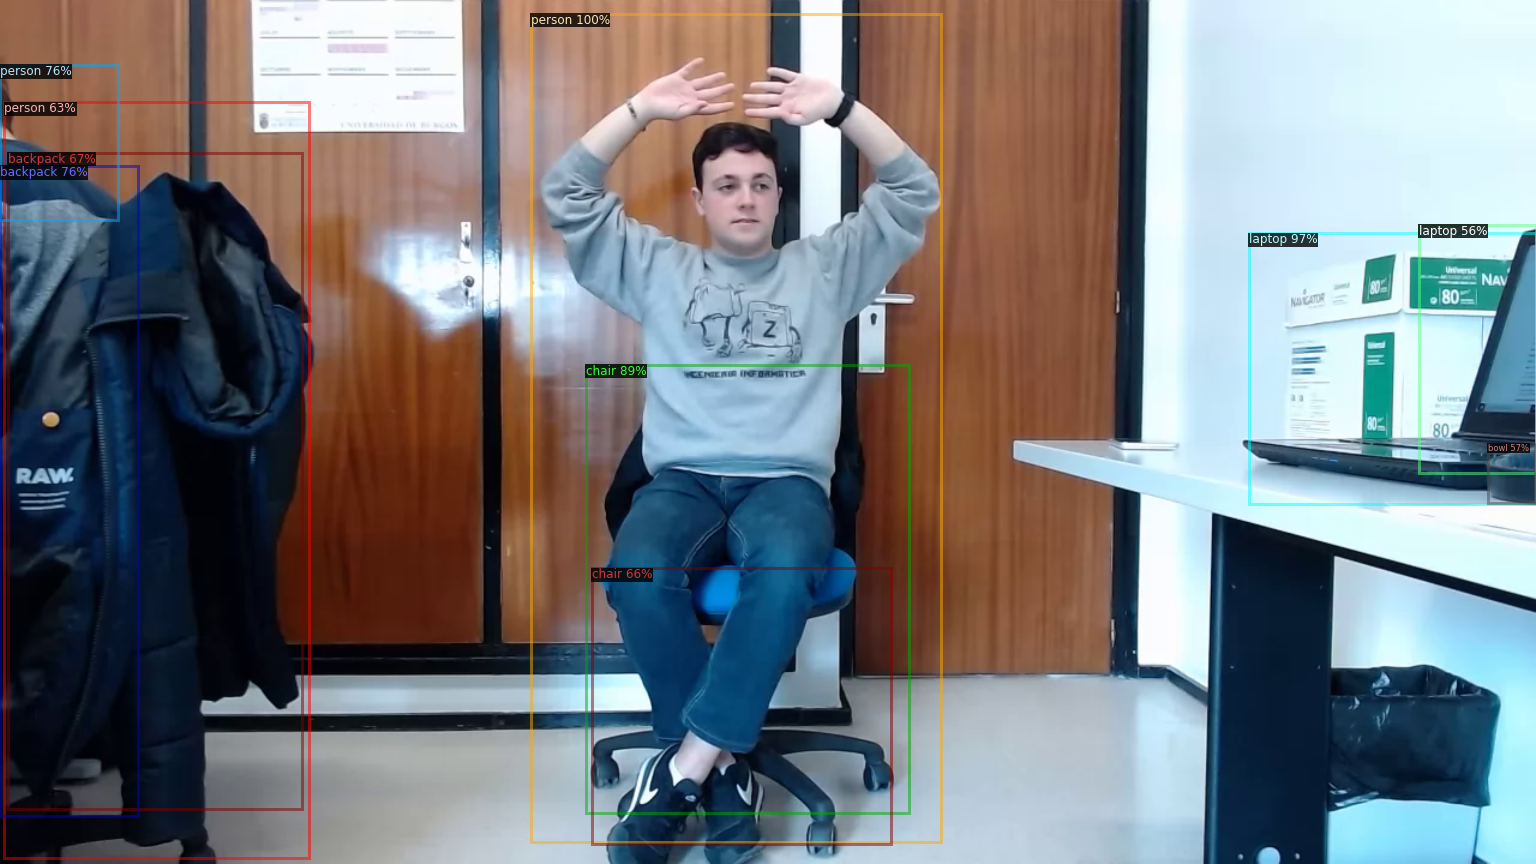
\includegraphics[width=1\textwidth]{faster_rcnn_R_50_C4_1x}
		\caption{Modelo de tipo COCO Detection with Faster R-CNN, faster\_rcnn\_R\_50\_C4\_1x.}
		\label{fig:faster_rcnn_R_50_C4_1x}
	\end{figure}
	\item COCO Detection with RetinaNet (Figura~\ref{fig:retinanet_R_101_FPN_3x}): modelos que detecta objetos y persona. Como se puede ver en la imagen de ejemplo la interpretación no es buena aun utilizando un \textit{threshold} alto.
	\begin{figure}[h]
		\centering
		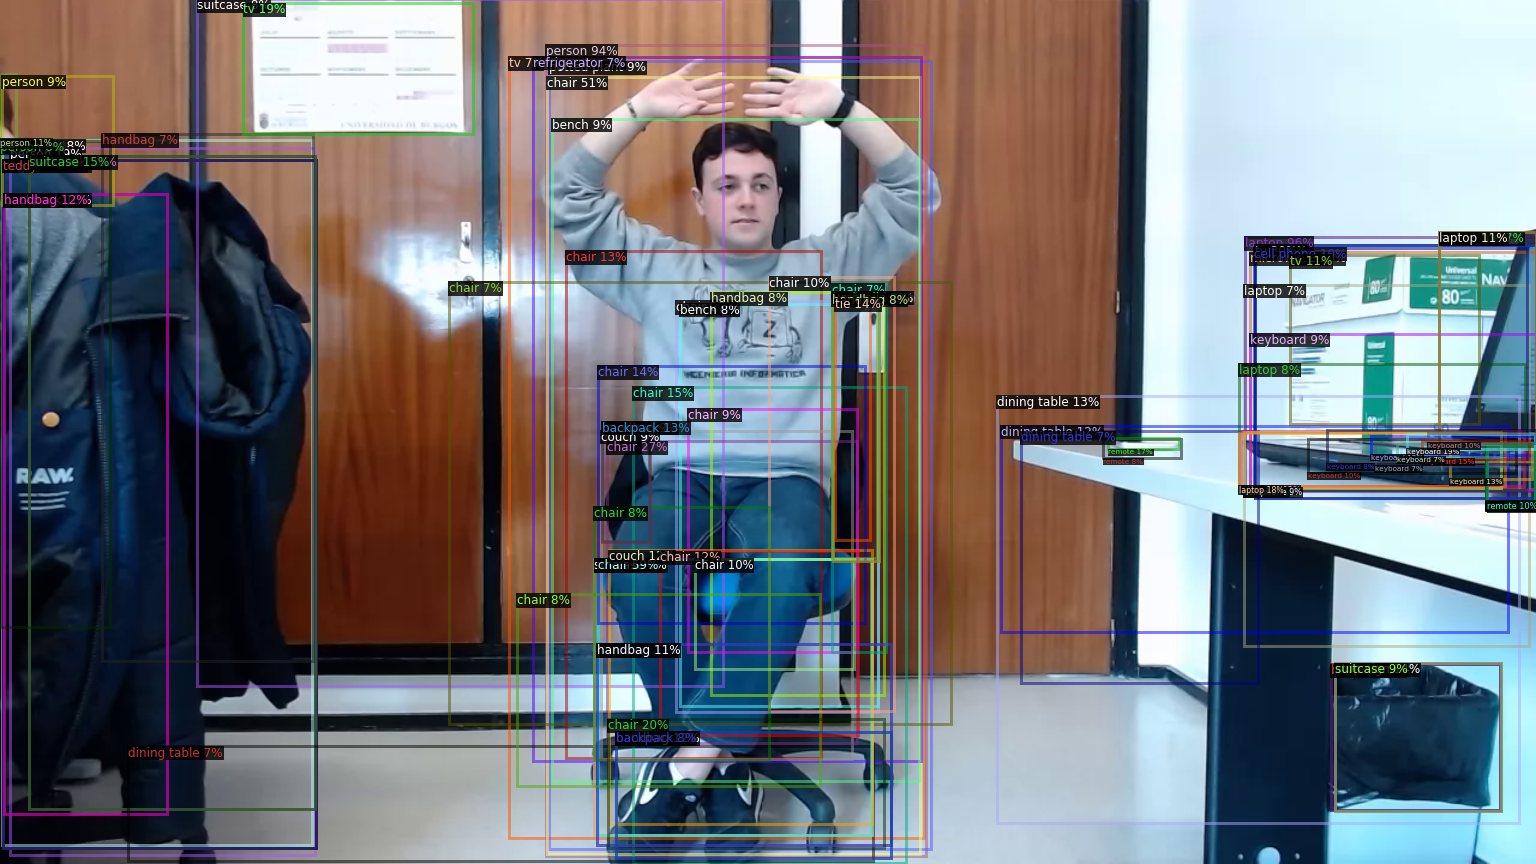
\includegraphics[width=1\textwidth]{retinanet_R_101_FPN_3x}
		\caption{Modelo de tipo COCO Detection with RetinaNet, retinanet\_R\_101\_FPN\_3x.}
		\label{fig:retinanet_R_101_FPN_3x}
	\end{figure}
	\item COCO Detection with RPN and Fast R-CNN: modelos que no se han conseguido probar ya que no siguen la misma estructura que el resto de modelos.
	\item COCO Instance Segmentation Baselines with Mask R-CNN (Figura~\ref{fig:mask_rcnn_R_50_DC5_3x}): modelos de detección de objetos y persona, con delimitación en el área ocupada.
	\begin{figure}[h]
		\centering
		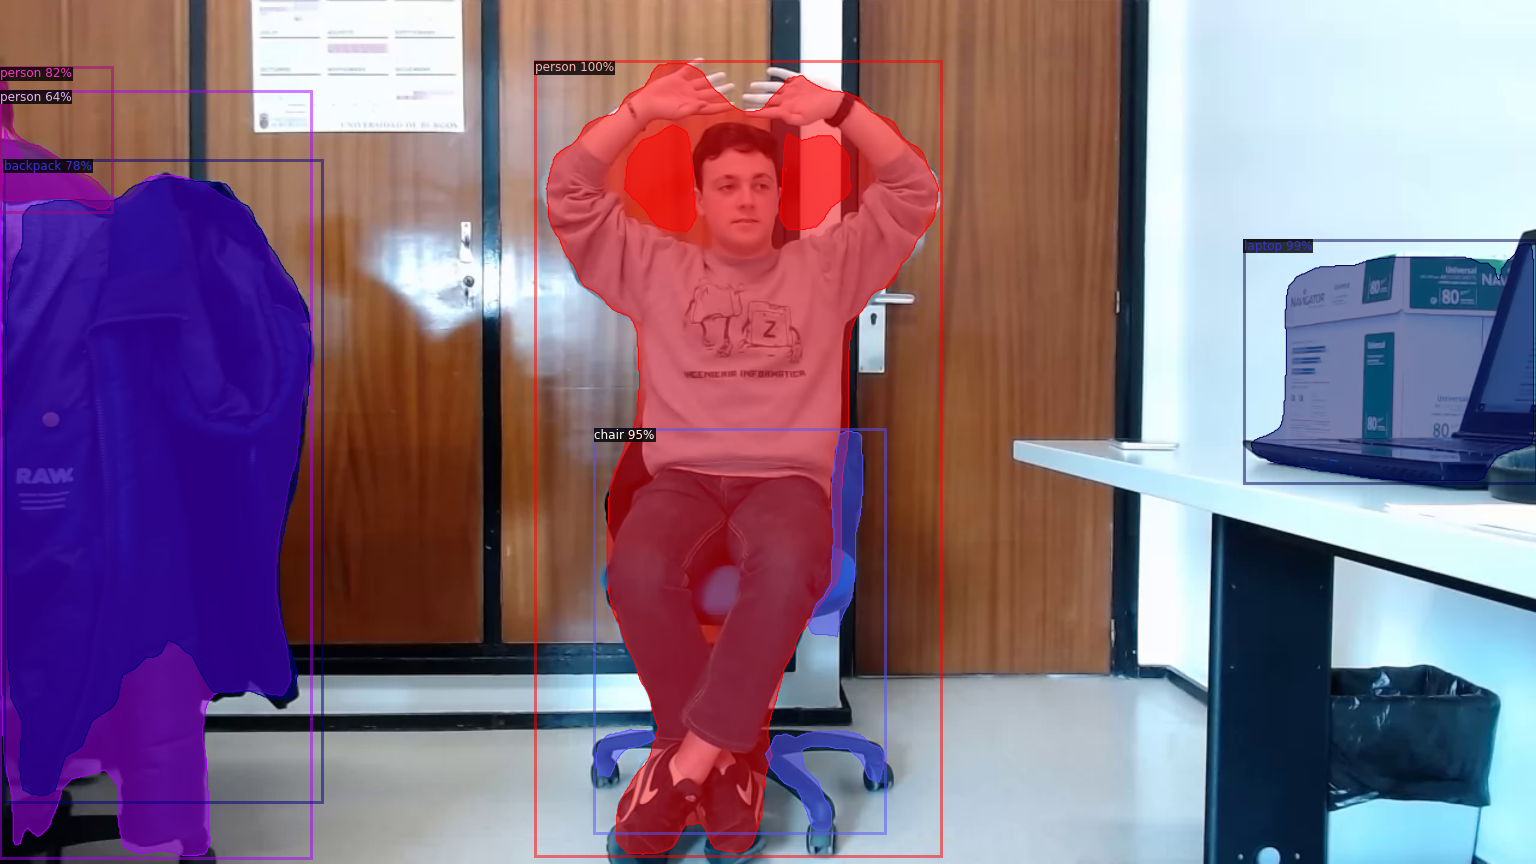
\includegraphics[width=1\textwidth]{mask_rcnn_R_50_DC5_3x}
		\caption{Modelo de tipo COCO Instance Segmentation Baselines with Mask R-CNN, mask\_rcnn\_R\_50\_DC5\_3x.}
		\label{fig:mask_rcnn_R_50_DC5_3x}
	\end{figure}
	\item COCO Person Keypoint Detection Baselines with Keypoint R-CNN (Figura~\ref{fig:keypoint_rcnn_R_101_FPN_3x}): modelos que detectan a las posiciones y unos puntos claves de ellas, estos puntos son nariz, ojos, orejas, hombros, codos, muñecas, cadera, rodilla y tobillos. Como se puede ver en la imagen de ejemplo, estos modelos predicen bastante bien la posición pero a veces detectan otras cosas como personas, por lo que se posteriormente se vio necesario un estudio sobre el \textit{threshold}.
	\begin{figure}[h]
		\centering
		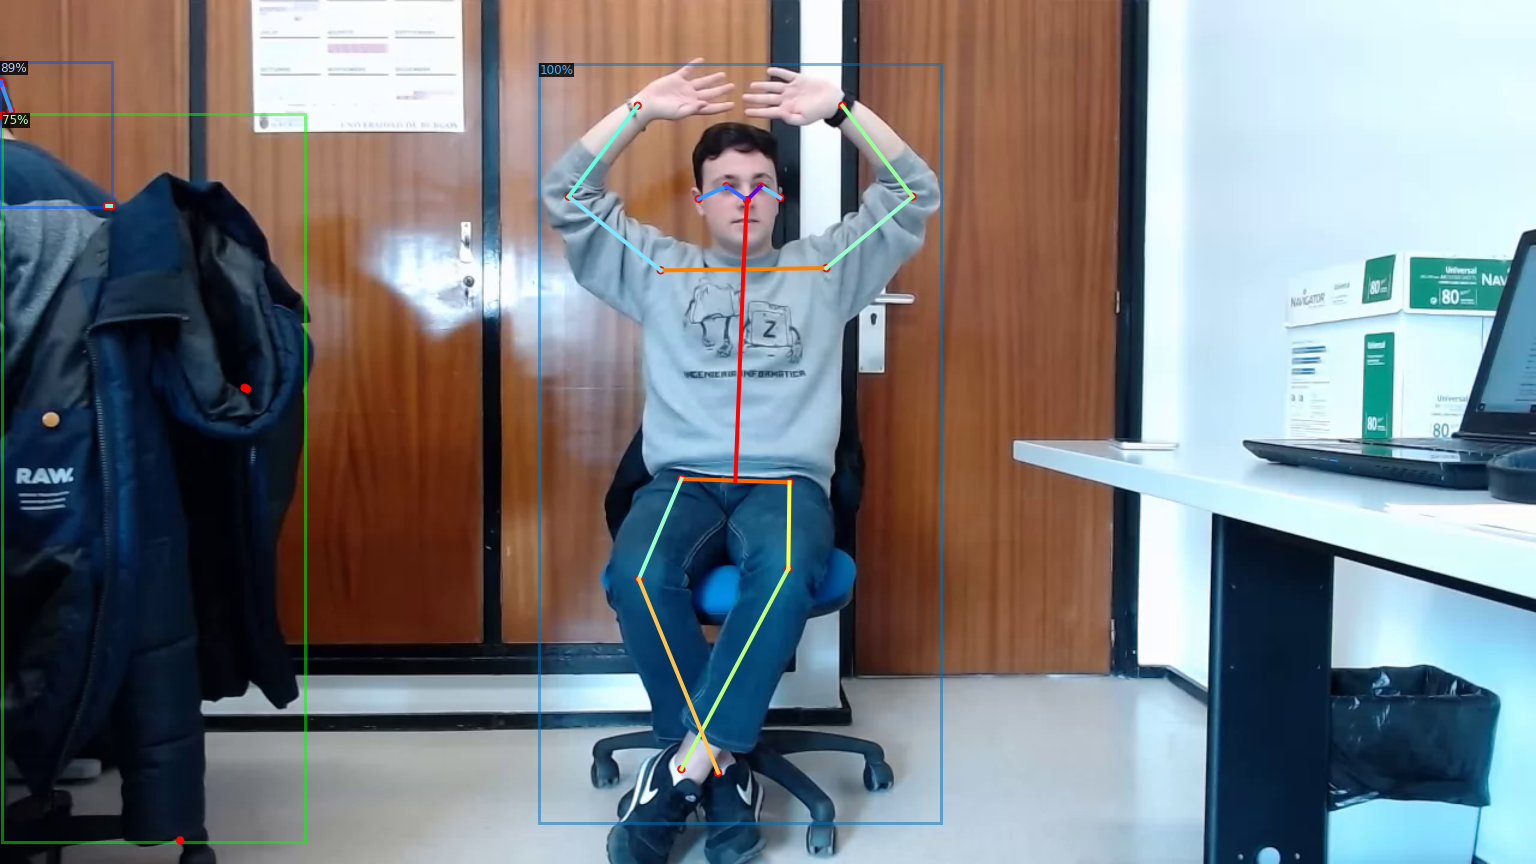
\includegraphics[width=1\textwidth]{keypoint_rcnn_R_101_FPN_3x}
		\caption{Modelo de tipo COCO Person Keypoint Detection Baselines with Keypoint R-CNN, keypoint\_rcnn\_R\_101\_FPN\_3x.}
		\label{fig:keypoint_rcnn_R_101_FPN_3x}
	\end{figure}
	\item COCO Panoptic Segmentation Baselines with Panoptic FPN (Figura~\ref{fig:panoptic_fpn_R_101_3x}): modelos que segmentación como COCO Instance Segmentation Baselines with Mask R-CNN, obtienen resultados muy parecidos.
	\begin{figure}[h]
		\centering
		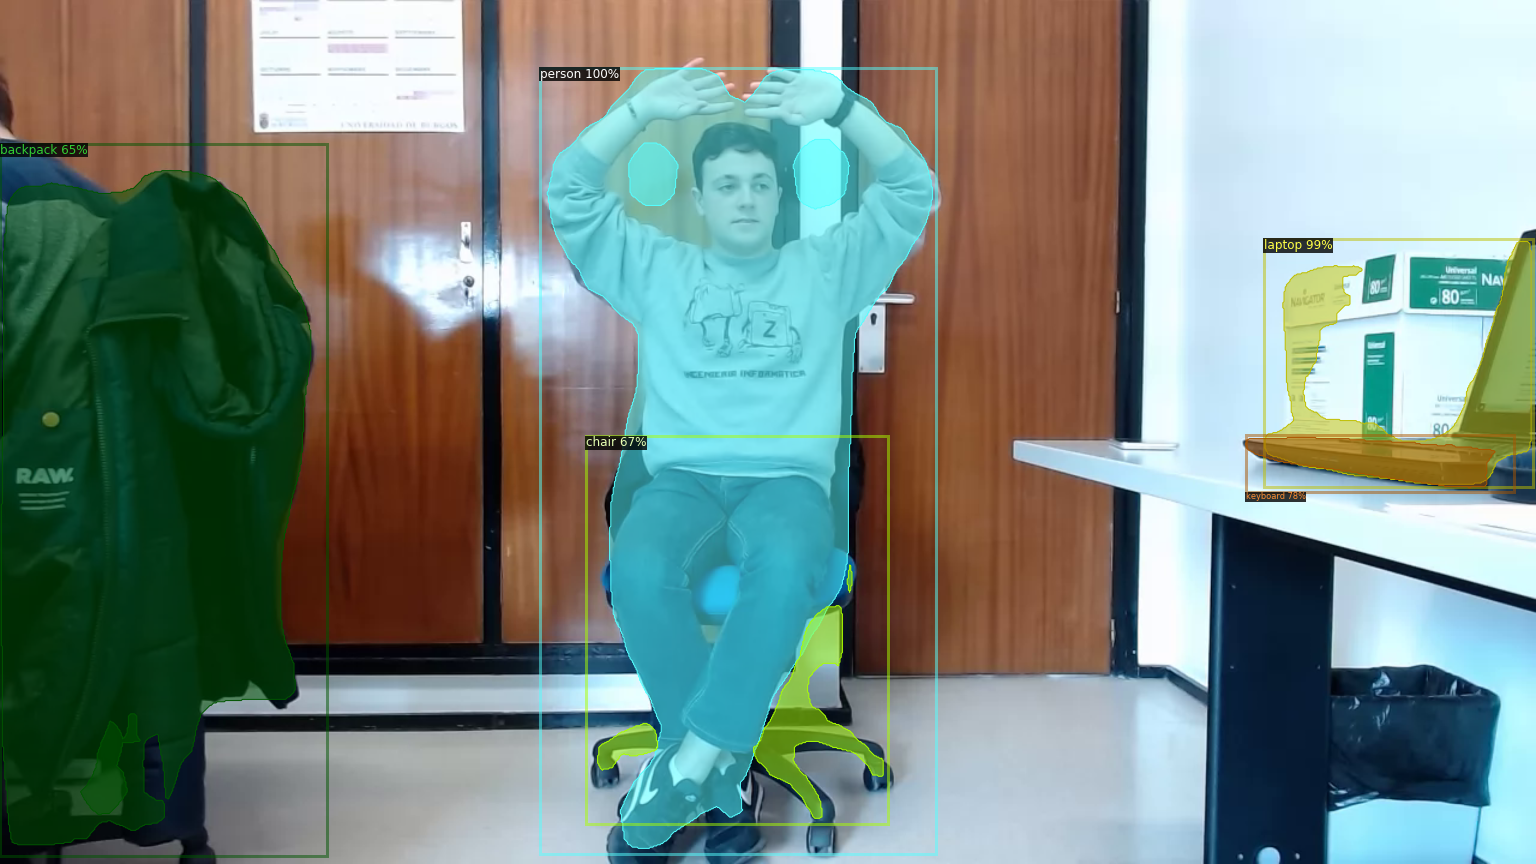
\includegraphics[width=1\textwidth]{panoptic_fpn_R_101_3x}
		\caption{Modelo de tipo COCO Panoptic Segmentation Baselines with Panoptic FPN, panoptic\_fpn\_R\_101\_3x.}
		\label{fig:panoptic_fpn_R_101_3x}
	\end{figure}
	\item LVIS Instance Segmentation Baselines with Mask R-CNN (Figura~\ref{fig:mask_rcnn_X_101_32x8d_FPN_1x}): modelos orientados a la detección de objetos, necesitan un \textit{threshold} bajo para detectar diversos objetos.
	\begin{figure}[h]
		\centering
		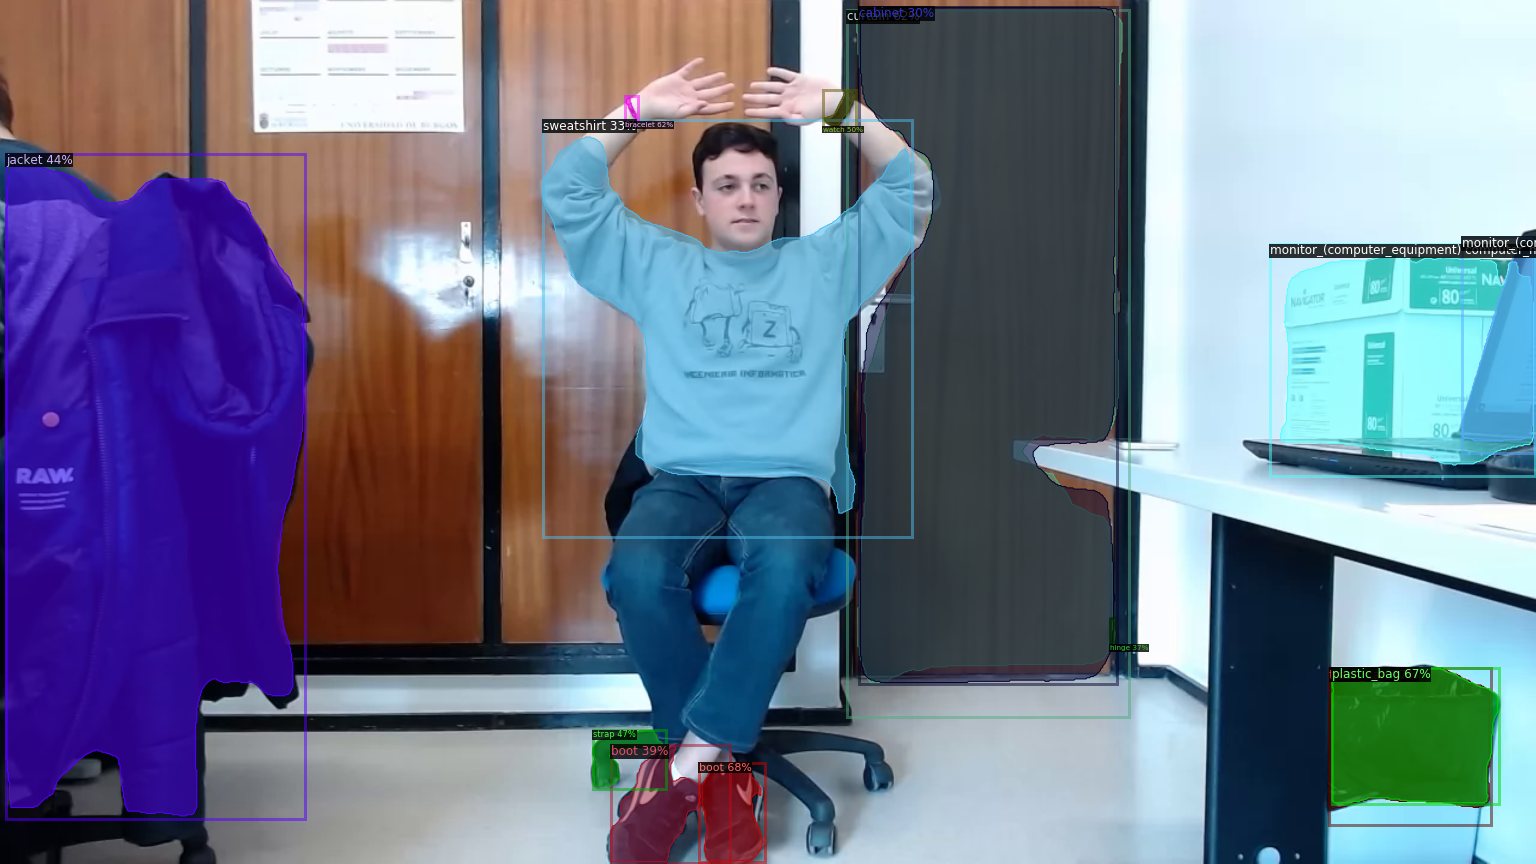
\includegraphics[width=1\textwidth]{mask_rcnn_X_101_32x8d_FPN_1x}
		\caption{Modelo de tipo LVIS Instance Segmentation Baselines with Mask R-CNN, mask\_rcnn\_X\_101\_32x8d\_FPN\_1x.}
		\label{fig:mask_rcnn_X_101_32x8d_FPN_1x}
	\end{figure}
	\item Por último se encuentran modelos como Cityscapes \& Pascal VOC Baselines, otras configuraciones y algoritmos de la primera versión de la herramienta \textit{Detectron}. Estos modelos son muy parecidos a los ya mostrados.
\end{itemize}

Con el estudio de todos los modelos existentes en \textit{Detectron2} se ha comprobado como los únicos modelos que sirven para el problema planteado son COCO Person Keypoint Detection Baselines with Keypoint R-CNN. Dentro de este tipo de modelos existen un total de 4 modelos distintos, para la elección del mejor de estos modelos se realizó otro estudio esta vez comprobando los tiempos de ejecución, ya que todos los modelos de este tipo realizan unas buenas predicciones (principalmente porque el problema es sencillo, al tener a la persona en el centro de la imagen con el mínimo de objetos de por medio).

Para realizar este estudio se analizó el tiempo de procesado e impresión de varios vídeos con cada uno de los modelos. Para ello se calculó estos valores para los 4 posibles modelos con un total de 7 vídeos. De este estudio se obtuvieron los resultados que se pueden ver en la tabla~\ref{tab:modelos}.

\begin{table}[h]
	\centering
	\resizebox{\columnwidth}{!}{
\begin{tabular}{l | rrrr}
	\toprule
	\textbf{Modelo} &     \textbf{T. Carga (s)} &       \textbf{T. Procesamiento (s)} &  \textbf{N. Fotogramas} &     \textbf{Frecuencia} \\
	\midrule
	keypoint\_rcnn\_R\_50\_FPN\_3x     &   9.783479 &  236.774504 &     1989 &  0.119042 \\
	keypoint\_rcnn\_R\_50\_FPN\_1x      &   8.562254 &  237.289880 &     1989 &  0.119301 \\
	keypoint\_rcnn\_R\_101\_FPN\_3x     &  13.017239 &  279.327051 &     1989 &  0.140436 \\
	keypoint\_rcnn\_X\_101\_32x8d\_FPN\_3x &  18.106832 &  422.024270 &     1989 &  0.212179 \\
	\bottomrule
\end{tabular}
}
\caption{Tabla con el estudio de los modelos de posición ordenado por ratio.}
\label{tab:modelos}
\end{table}

Como se pueden observar, los datos obtenidos para los modelos son muy parecidos, sobre todo para los dos con mejor frecuencia. Tras observar estos datos se decidió elegir al modelo keypoint\_rcnn\_R\_50\_FPN\_3x (es además el modelo con el que se hicieron las primera pruebas y con el que se decidió a \textit{Detectron2} como herramienta para detectar el movimiento) para utilizarlo en el resto del proyecto. Además, en este estudio se ha podido comprobar que los modelos trabajan correctamente sea cual sea el tipo de ropa que lleve la persona o si pasa un objeto por medio de la imagen (normalmente la posición es correcta, pero como se comentará más adelante a veces algunos fotogramas no son correctos), como se pueden ver en la figuras~\ref{fig:chaqueta} y~\ref{fig:caja}.

\begin{figure}[h]
	\centering
	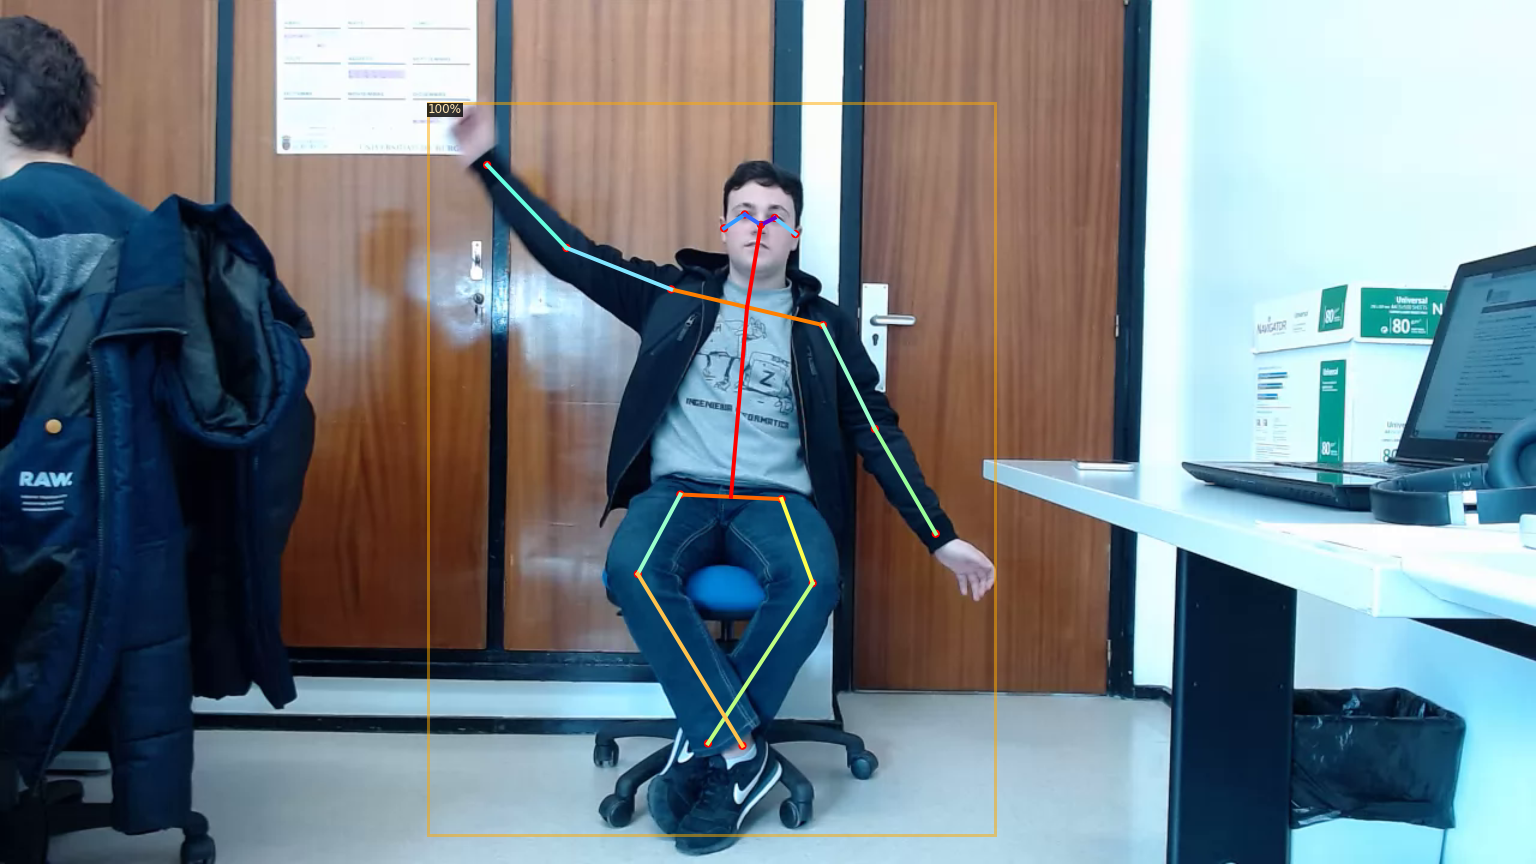
\includegraphics[width=1\textwidth]{chaqueta}
	\caption{Prueba con chaqueta.}
	\label{fig:chaqueta}
\end{figure}

\begin{figure}[h]
	\centering
	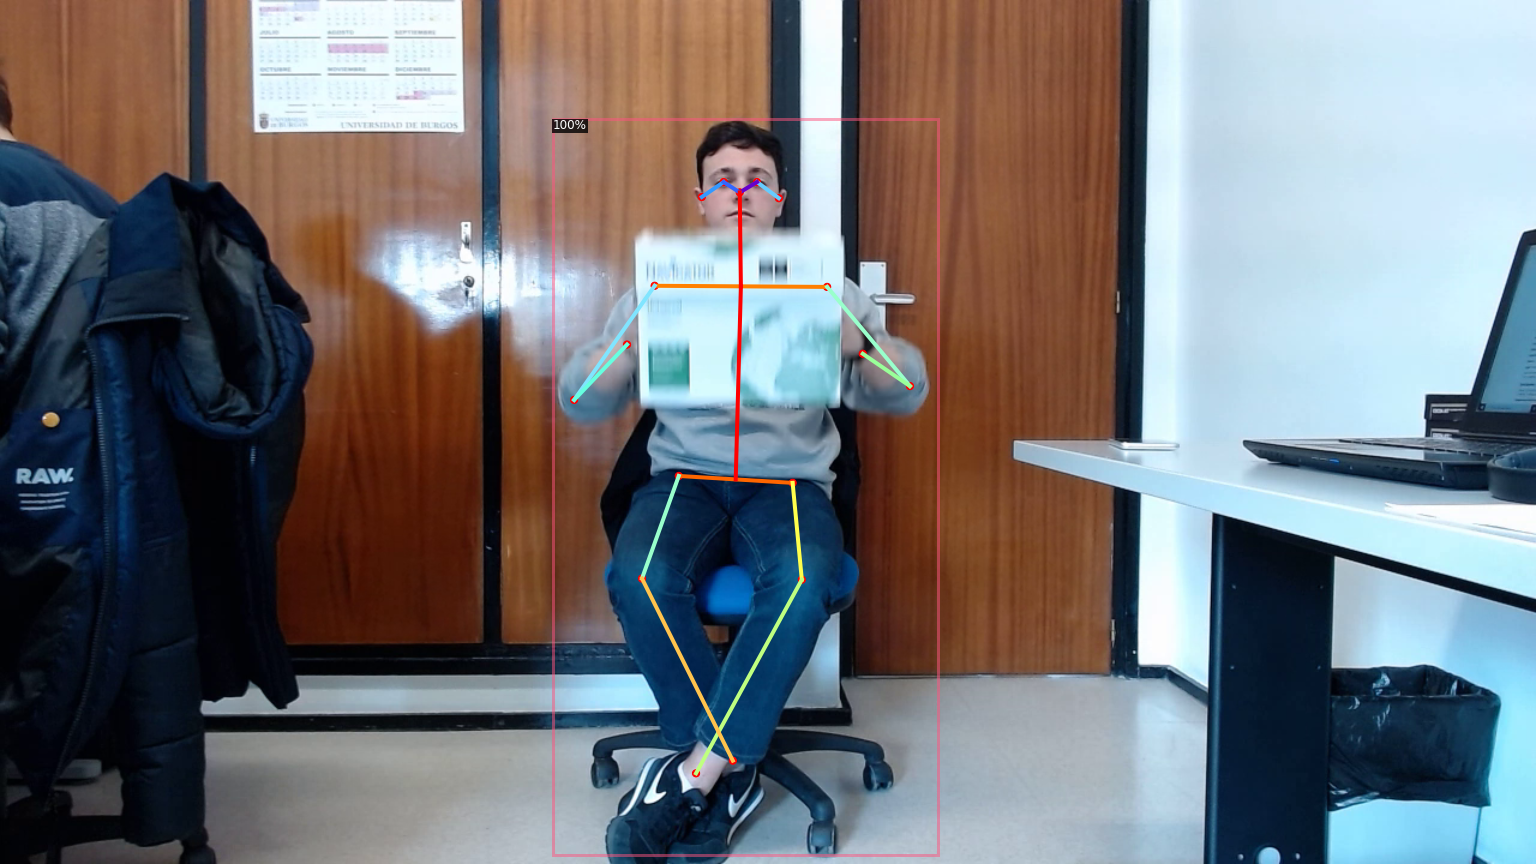
\includegraphics[width=1\textwidth]{caja}
	\caption{Prueba con un objeto de por medio.}
	\label{fig:caja}
\end{figure}


\subsection{Definición del \textit{threshold}}
Como se ha comentado en el apartado anterior, es necesario definir un \textit{threshold}, que es un valor entre 0 y 1 que define la sensibilidad del modelo al detectar, es decir, con valores cercanos a 0 el modelo tiende a detectar más elementos (muchos de ellos erróneos) y cuanto más cercano a 1 menos sensible es, solo detectando los elementos más claros. Sobre este valor se ha realizado un estudio de posibles valores, estos valores probados han sido 0.3, 0.5, 0.75 y 0.99.

Con valores bajos del \textit{threshold} se observa que se detectan cosas que no son personas, o se detectan personas que no salen completas en la imagen, como se puede observar en el figura~\ref{fig:pruebaCon0.3}. Esto ocurre con los valores 0.3, 0.5 y 0.75 que dan la misma salida. Sin embargo, con el valor 0.99, como se puede ver en la figura~\ref{fig:pruebaCon0.99}, se obtienen muy buenos resultados detectando únicamente a la persona que aparece en el centro de la imagen, con la posición exacta en todos los puntos.

\begin{figure}[h]
	\centering
	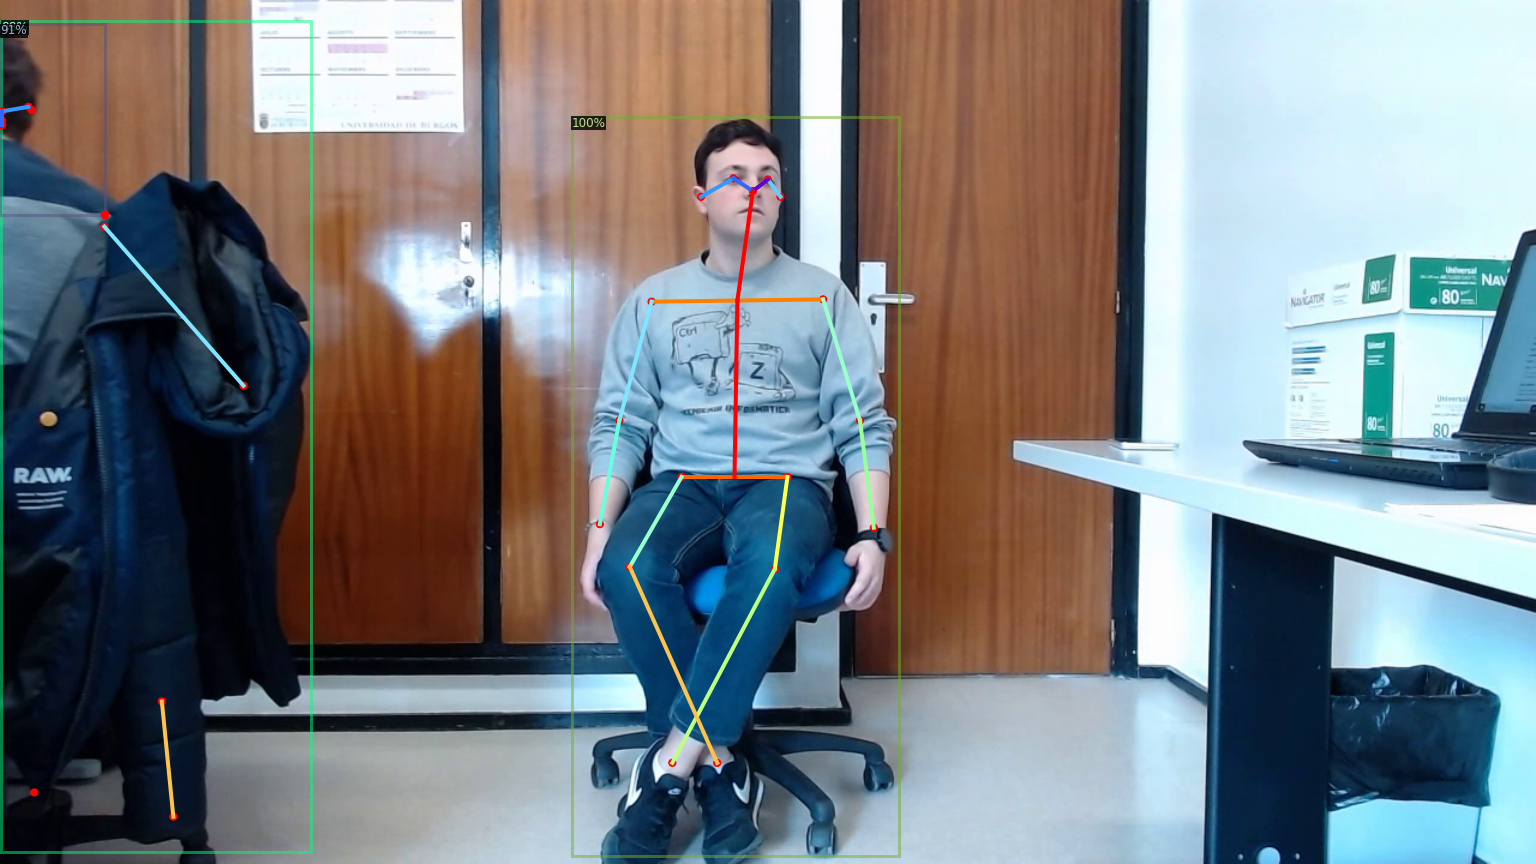
\includegraphics[width=1\textwidth]{pruebaCon0.3}
	\caption{Prueba con \textit{threshold} a 0.3.}
	\label{fig:pruebaCon0.3}
\end{figure}

\begin{figure}[h]
	\centering
	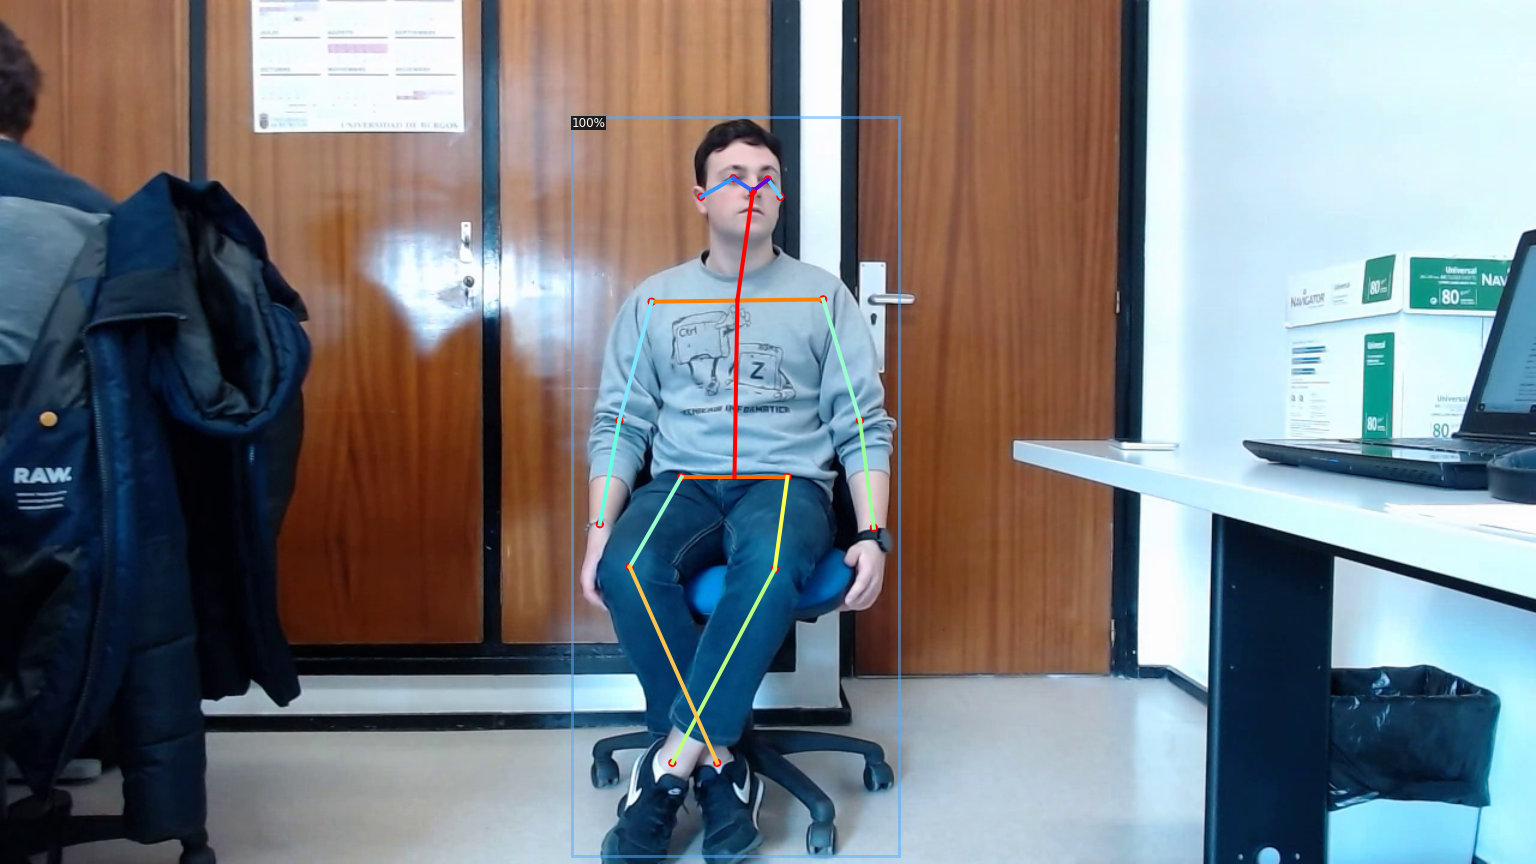
\includegraphics[width=1\textwidth]{pruebaCon0.99}
	\caption{Prueba con \textit{threshold} a 0.99.}
	\label{fig:pruebaCon0.99}
\end{figure}

\subsection{Problemas surgidos}
Como se ha comentado a lo largo del apartado, han surgido distintos problemas que se pueden resumir en:
\begin{itemize}
	\item Problema con los modelos COCO Detection with RPN and Fast R-CNN que al no tener la misma estructura que el resto de modelos de \textit{Detectron2} no se ha podido probar.
	\item Se intentó almacenar los vídeos procesados pero por problemas con \textit{OpenCV} no se pudo guardar en esta etapa.
\end{itemize}

\section{Cálculo de características}
Una vez se seleccionó el modelo que se iba a utilizar durante todo el proyecto y se determinó el parámetro \textit{threshold} de los modelos, el siguiente paso es la interpretación de las salidas del modelo. Y después de haber interpretado con el modelo de \textit{Detectron2} una posición ser capaces de calcular características que definan de la mejor manera los datos.
\subsection{Interpretación de las predicciones}
Si se analiza la salida tras predecir un imagen con el predictor creado (DefaultPredictor) se observa que devuelve un diccionario con una única entrada llamada ``instances'' donde se almacena toda la información. Dentro de la instancia existen los siguientes apartados:
\begin{itemize}
	\item \textit{pred\_boxes}: Boxes, estructura propia de \textit{Dectectron2} donde se almacenan límites de donde entiende que está la persona en un \textit{tensor}, si se ha detectado más de una persona este Boxes estará creado por varios \textit{tensors}.
	\item \textit{scores}: \textit{tensor} con las probabilidades de que los elementos sean personas. Es este el valor que se compara con el \textit{threshold} para ver si se toma o no como una persona. Si existe más de un valor estos están ordenados de mayor a menos, este es el orden que se sigue en el resto de valores.
	\item \textit{pred\_classes}: \textit{tensor} con el índice de la clase, en este caso todos los elementos son 0 ya que solo detecta personas, que se identifican con este índice.
	\item \textit{pred\_keypoints}: \textit{tensor} con todos los puntos clave de cada elemento (persona) detectada. De cada elemento detectado, si la predicción ha sido correcta, se obtienen un total de 17 puntos, con sus valores x e y. Después de investigar el posicionamiento de estos puntos se puede decir, como se ve en la figura~\ref{fig:puntos}, que los puntos representan (teniendo en cuenta que se han detectado todos los puntos y que la persona está mirando de frente al objetivo):
	\begin{itemize}
		\item 0: nariz.
		\item 1 y 2: ojo izquierdo y derecho.
		\item 3 y 4: oreja izquierda y derecha.
		\item 5 y 6: hombro izquierdo y derecho.
		\item 7 y 8: codo izquierdo y derecho.
		\item 9 y 10: muñeca izquierda y derecha.
		\item 11 y 12: parte izquierda de la cadera y derecha.
		\item 13 y 14: rodilla izquierda y derecha.
		\item 15 y 16: tobillo izquierdo y derecho.
	\end{itemize}
\end{itemize}

\begin{figure}[h]
	\centering
	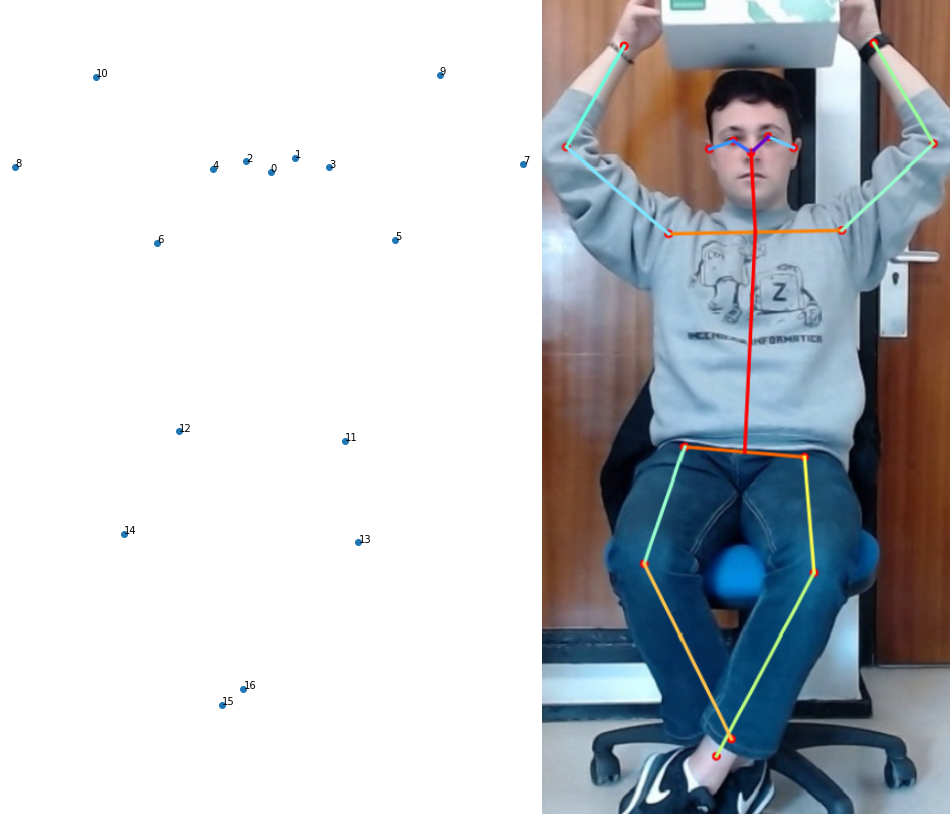
\includegraphics[width=0.5\textwidth]{puntos}
	\caption{Puntos clave predichos con el modelo junto con la etiqueta con su orden.}
	\label{fig:puntos}
\end{figure}
\subsection{Clase de posición}
Una vez se conoce la salida de las predicciones se puede usar esta para obtener más información de la posición de la persona, que en futuras etapas fue usada para la comparación de posiciones. Por ello se creó una clase que almacena todos los puntos detectados además de realizar cálculos para extraer más características.

Para poder obtener más información sobre los puntos se crearon una serie de funciones que permiten el cálculo de:
\begin{itemize}
	\item Cálculo de puntos medios. Este cálculo se realiza para obtener el punto inferior del cuello que se calcula como el punto medio de la recta que une los dos hombros y se utiliza también para calcular el punto central de la cadera a partir de su punto izquierdo y derecho.
	\item Cálculo de la distancia entre puntos. Este punto se ha realiza sobre todos los pares de puntos unidos. Se pueden utilizar para intuir profundidades.
	\item Cálculo de los ángulos en grados. Este cálculo se ha realizado en todas las combinaciones posibles (conjunto de 3 puntos consecutivos), ya que se cree que son las características que más información van a aportar debido a que no dependen de ningún otro valor como puede ser la profundidad a la que está el paciente, su altura...
\end{itemize}

Como se comentó en apartados anteriores, una vez se tienen los puntos se ha de realizar una serie de comprobaciones para saber si las posiciones son válidas:
\begin{itemize}
	\item Si existe más de una persona detectada se selecciona la primera, ya que es la que tiene un mayor \textit{score} y por lo tanto el modelo cree que puede ser con mayor probabilidad una persona.
	\item Si una predicción no dispone de todos los puntos no se tiene en cuenta. En la práctica con las pruebas que se han realizado esto solo pasa cuando se pasa un objeto por ciertos puntos del cuerpo, cuando ocurre estos hay algunos fotogramas, muy pocos, que no detectan todos los puntos.
	\item Se compara el fotograma actual con un conjunto de fotogramas anteriores, si la diferencia entre ellos son muy grandes se descarta el fotograma ya que se entiende que el modelo no ha procesado bien la imagen. Este suceso pasa también cuando se pasa un objeto por alguna parte del cuerpo, ya que cuando esto ocurre a veces algunos fotogramas dan predicciones erróneas que se pueden detectar con una simple comparación con una ventana deslizante de posiciones.
\end{itemize}

